\chapter{Introduction}
\label{sec:intro}

\cleanchapterquote{Finance is the art of passing currency from hand to hand until it finally disappears.}{Robert W. Sarnoff}{(1918-1997)}

This introductory chapter starts, in Section \ref{sec:intro:motivation}, with the motivation on the option pricing, that have been the starting point for this work. We will briefly discuss about the existing works we used to develop this project. Then, in Section \ref{sec:intro:description}, the FX-TARN product is presented. In Section \ref{sec:intro:term_sheet}, an example of term sheet illustrates this exotic product. Finally, the chapter concludes with an overview of the thesis in Section \ref{sec:intro:overview}.

\section{Motivation}
\label{sec:intro:motivation}
This project was born during my internship in market risk management at Pictet, a swiss private bank. In fact, I had to reprice FX-TARN to evaluate the risk on this product. The first approach was to price it with Monte Carlo simulations. However, the computational cost was very expensive. Several numbers of research brought me to the paper of \citeauthor{LS15} \citeyearpar{LS15} \cite{LS15}, in which they develop a Finite Difference (FD) method for Black-Scholes model. 

It is well known that the assumptions under Black-Scholes model are too restrictive with respect to the market. Indeed, the log-normality of the returns and the path continuity are contradicted by the analysis of the financial data. We can clearly identify jumps in financial time series. In addition, the implied volatility presents in general a negative skew which means that the returns distribution is more leptokurtic (fat tails) than the normal one. This can be due effectively to the jumps in the market prices, accentuated during the economic crises.

To go beyond the Black-Scholes model and avoid inconsistencies with the markets, we can model stock price with exponential L\'evy processes. There are two different classes of L\'evy models used in this thesis, the jump-diffusion (finite activity) models which are extension of Black-Scholes model including jumps, and pure jump (infinite activity) models which model the asset price by infinitely many small jumps. The advantage of these models is that they capture
the volatility smile structure. 

The first part of the study was thus to enlarge the Finite Difference (FD) method proposed by \citeauthor{LS15} to the L\'evy processes with jumps. This generalization involves the L\'evy measure characterizing the jumps. This leads to large complexities in the implementation of the method and then the computational time grows up with the complexity. Therefore the question was how to boost the pricing engine. The Computational Finance lesson given by the Prof. \citeauthor{Nob15} \cite{Nob15} in collaboration with Prof. Pulido and Kressner from the Swiss Institute of Technology Lausanne (EPFL), gives me the idea to solve the problem with Fast Fourier Transform (FFT). At the end, the solution was found in the Convolution method proposed by \citeauthor{Lor+08} \citeyearpar{Lor+08} \cite{Lor+08}, where they apply a FFT based method to the early exercised option like Bermudan or American options. T hen, the combination of the methods of \citeauthor{LS15} and \citeauthor{Lor+08} allows us to develop our own method to price FX-TARN with the FFT approach.

To achieve this project, it was natural to call the Prof. Fabio Nobile, who is a specialist of numerical analysis in partial differential equations (PDE), and the Prof. Julien Hugonnier, who taught me the pricing of financial derivatives. Thank's to them for their useful supervision.

\section{FX-TARN Description}
\label{sec:intro:description}
First of all, the foreign exchange market, also called Forex, FX, or currency market, is an over-the-counter OTC market (trading directly between two parties without supervision) for the trading of the currencies. This is the largest financial market in the world in term of trading volume, with trillions of dollars worth of transactions each day. 

Thus, an FX Target Accrual Redemption Note (FX-TARN) is an exotic financial product on a currency pair (e.g. USD/CHF) very popular in Asia. It allows an investor to accumulate, over a predefined period of time, an amount of cash until a certain \textit{target accrual level} $U$ is reached. More precisely, the contract between the bank and the client imposes positive and negative cash flows on scheduled dates (called \textit{fixing dates}). These cash flows can take the form of Call or Put option payoffs. For example, in a so called FX TARN Accumulator, a positive cash flow is a Call option payoff and a negative cash flow is a Put option payoff multiplied by a gear factor $g$ that penalizes the client versus the bank. In the case of an FX TARN Decumulator, the roles of the Call options and Put options are inverted.

Hence, we can replicate this exotic option with a series of FX call options (resp. FX put options) with strike $K$, that the bank sells to a client, and at the same time a series of FX put options (resp. FX call options) with the same strike $K$, that the bank buys from the client. The scheduling is defined by a number of fixing dates $t_1,t_2,\ldots,t_N$ that correspond to the options expiry dates.

Finally, a redemption condition is done on the accumulated positive amount. In fact, the product knocks-out if the total sum of the positive cash flows exceeds the given target $U$. We will study three types of knock-out when the target $U$ is breached:
\begin{my_list_item}
\item \textbf{No Gain :} the last payment is disallowed when the target $U$ is breached,
\item \textbf{Part Gain :} only a part of the payment is allowed such that only the target is paid,
\item \textbf{Full Gain :} the last payment is allowed when the target $U$ is breached. 
\end{my_list_item}

This pure speculative financial product is very risky and enjoys the Chinese. Investing in such derivative is like playing in a casino where the casino has a bounded risk while the client can lose a lot. Indeed, the knock-out condition cut the loss of the bank point of view when the client wins too much money.

\subsubsection*{Payoff Definition}
\label{sec:intro:Payoff}
We will use the following notation:
\begin{my_list_item}
\item $S(t)$ : FX rate at time $t$,
\item $K$ : strike(s) (could be different for each fixing dates),
\item $t_0$ : today's date,
\item $t_1,t_2,\ldots,t_N$ : fixing dates,
\item $U$ : target accrual level,
\item $A(t)$ : accumulated amount of positive cash-flow at time $t$,
\item $N_f$ : Notional amount per fixing date.
\end{my_list_item}

In order to understand a bit more the running of the FX TARN, we will explain in more detail the payoff. 

On each fixing date $t_n, n = 1,\ldots,N,$ if the target level $U$ is not breached by the accumulated amount $A(t_n)$, we can define the positive payoff per unit of notional foreign amount by
$$\tilde{C}^\text{pos}_n \equiv \tilde{C}^\text{pos}(t_n) = \max(\beta(S(t_n)-K),0), $$
and the negative payoff by
$$\tilde{C}_n^\text{neg}\equiv \tilde{C}^\text{neg}(t_n) = -g \times \max(\beta(K-S(t_n)),0),$$
where $\beta$ is the investor strategy, i.e. with $\beta = 1$ he buys Call options, and with $\beta = -1$ he buys Put options. If he buys Call options, we say that he accumulates the domestic currency and in the other case, if he buys Put options, we say that he decumulates. This gives the respective name of FX TARN Accumulator or Decumulator.

Denote $t_{\tilde{N}}$ the first fixing date before maturity $T$ on which the target level $U$ is breached by the total accumulated positive cash flow $A(t_n), n = 1,\ldots,N,$ (without decumulating with negative cash flows!). In other words,
\[\tilde{N}=\min\{n: A(t_n)\geq U\},\qquad n = 1,2,\ldots,N.\]
The three different knock out conditions, No Gain, Part Gain and Full Gain means that if the accumulated amount breaches the target $U$ in the No Gain case, the last cash flow is not payed since in the Full Gain case it is payed and then the product is killed. In the Part Gain case, the last cash flow completes the target amount and then the deal is over.

For $t_n = t_{\tilde{N}}$:
$$A(t_n) = \begin{cases}
A(t_{n-1}), & \text{No Gain,}\\
U, &\text{Part Gain,}\\
A(t_{n-1}) + \tilde{C}_n^\text{pos},&\text{Full Gain.}
\end{cases}$$

For $t_n>t_{\tilde{N}}$:
$$A(t_n) = A(t_{\tilde{N}}.$$

If the target $U$ is not breached, we set $\tilde{N} = N$. Then for $t_n \leq t_{\tilde{N}}$ we can write the positive cash flow on $t_n$ as
\begin{equation}\label{eq:TARN:gain}
C^\text{pos}(S(t_n),A(t_{n-1})) = \tilde{C}^\text{pos}_n\times \left(\mathbf{1}_{\left\{A(t_{n-1}))+\tilde{C}^\text{pos}_n<U\right\}}+W_n\times\mathbf{1}_{\left\{A(t_{n-1})+\tilde{C}^\text{pos}_n\geq U\right\}}\right),
\end{equation}
where 
\[W_n = \begin{cases}
0, &\text{for No Gain,} \\
\frac{U-A(t_{n-1})}{\beta\times(S(t_n)-K)}, & \text{for Part Gain,}\\
1, &\text{for Full Gain.}
\end{cases}\]

Note that $C^\text{pos}=0$ for $t_n>t_{\tilde{N}}$. The negative cash flow does not count in the knock-out condition but will also knock-out by the same redemption event. Therefore we have that
\begin{equation}\label{eq:TARN:loss}
C^\text{neg}(S(t_n),A(t_{n-1})) = \tilde{C}_n^\text{neg}\times \left(\mathbf{1}_{\left\{A(t_{n-1}))+\tilde{C}^\text{pos}_n<U\right\}}+W_n\times\mathbf{1}_{\left\{A(t_{n-1})+\tilde{C}^\text{pos}_n\geq U\right\}}\right)
\end{equation}

In Figure \ref{fig:cash-flow}, we can see the plot of the positive cash flow $C(S(t),A(t^-)) = C(S,A)$ that counts in the accumulated amount and produces jumps in the price on each fixing date.
\begin{figure}[!htb]
\centering
	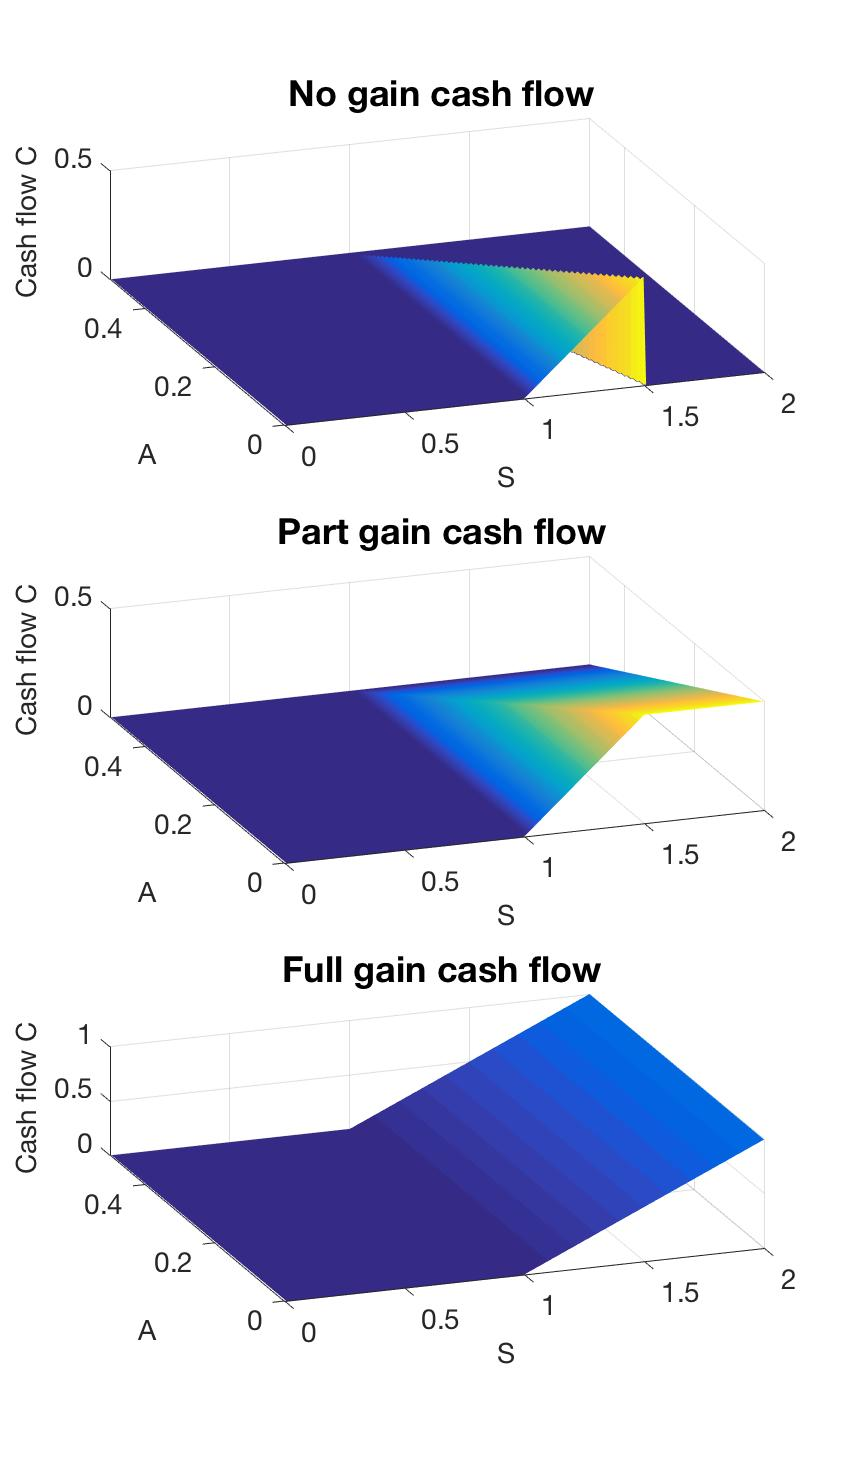
\includegraphics[scale = 0.25]{gfx/Cash-flow}
	\caption{Positive cash flow that produces jump on a fixing date for different type of knock-out.}
	\label{fig:cash-flow}
\end{figure}

Finally, the net present value of FX-TARN in domestic currency for FX rate realization $\mathbf{S} = (S(t_1),S(t_2),\ldots,S(t_N))$ is
\begin{equation}\label{eq:intro:pv}
P(\mathbf{S}) =N_f \times \sum_{n=1}^N\frac{C^\text{tot}(S(t_n),A(t_{n-1}))}{B_d(t_0,t_n)}, \qquad A(t_0)=0,
\end{equation}
where $B_d(t_0,t_n)^{-1}$ is the domestic discounting factor from $t_n$ to $t_0$ and 
$$C^\text{tot} = C^\text{pos}(S(t_n),A(t_{n-1}))+C^\text{neg}(S(t_n),A(t_{n-1}))$$ 
is the total cash flow at time $t_n$. Remark that a positive cash flow can not appears in the same time of a negative cash flow. Then the total cash flow is either positive or negative.

\section{Example of Term Sheet}
\label{sec:intro:term_sheet}
In this section, we will give an example of a particular TARN called \textit{"Leveraged Foreign Exchange Target Accrual Redemption Note with Full Settlement"}, i.e. Full Gain FX-TARN with gear factor. The term sheet has the following form.

\begin{longtable}{|l|l|} 
\hline
\textbf{USD/CHF FX-TARN} & \textbf{Key Characteristics of the Transaction} \\
\hline 
\hline
Instrument Type & Leverage FX Target Accrual Redemption Note (TARN) \\
\hline
Trade Date & 23 May 2017\\
\hline
Buyer of CHF & The Bank \\
\hline
Buyer of USD & The Client \\
\hline
Underlying & USD/CHF Foreign Exchange rate\\
\hline
Notional Amount & USD 2'080'000.00 \\
&(versus maximum notional amount USD 4'160'000.00)\\
\hline
Notional Amount & USD 40'000.00\\
per Fixing Date &(versus Leveraged Accrual Amount USD 80'000.00)\\
\hline
Leverage factor &2\\
\hline
Initial Spot Price & 0.9730 CHF per USD\\
\hline
Strike Price & As per date schedule below\\
\hline
Target Redemption Level & 0.4 CHF per 1 USD\\
\hline
Weekly Gains & On each Fixing Date, \\
& $\bullet$ If USD/CHF > Strike Price :\\
& \qquad Weekly Gains = USD/CHF - Strike Price\\ 
& $\bullet$ Otherwise :\\
& \qquad Weekly Gains = 0 CHF\\
\hline
Cumulated Gains & In respect of any Fixing Date, the Weekly Gains \\
& on that Fixing Date plus the sum of all Weekly \\
& Gains in respect of all previous Fixing Dates.\\
\hline
Redemption Event & A Redemption Event is deemed to have occurred \\
& if the Cumulated Gains (including the present fixing)\\ 
& is greater than or equal to the Target Redemption Level\\ 
& on any Fixing Date.\\
\hline
Expiration Date & 22 May 2018 \\
\hline
Fixing Reference & Weekly (Business Days)\\
\hline
Fixing Dates & 52 Fixings (see Schedule below)\\
\hline
Profile on Fixing Date & In respect of each Fixing Date :\\
& \textbf{1)} If no Redemption Event occurs and the Fixing Price is :\\
& $\quad\bullet$ At or above the Strike Price, the Client will buy from \\
& \qquad the Bank the Accrual Amount at the strike price : \\
& $\hspace{2cm}$ \textbf{Strike Price x Accrual Amount}\\
& Or \\
& $\quad\bullet$ Below the Strike Price, the Client will buy from the \\
& \qquad Bank the Leveraged Accrual Amount at the Strike  \\
& \qquad Price:\\
& $\hspace{1cm}$ \textbf{Leveraged Factor x Strike Price x Accrual Amount}\\
& \textbf{2)} If a Redemption Event occurs :\\
& $\quad\bullet$ The Client will buy from the Bank the Accrual Amount \\
& \qquad at the Strike Price for the Fixing Date that Redemption \\
& \qquad Event is deemed to have occurred : \\
& $\hspace{2cm}$ \textbf{Strike Price x Accrual Amount}\\
& $\quad\bullet$ The product is then knocked out for all remaining\\ 
& \qquad subsequent Fixings. There will be no further\\ 
&\qquad obligations between the Client and the Bank. \\
\hline
Schedule & \\
& \qquad\qquad$\begin{array}{|c|c|c|} 
\hline
\textbf{Fixing} & \textbf{Fixing Date} & \textbf{Strike Level} \\
\hline 
1 & 30 \text{ May } 2017 & 0.9275\\
2 & 6 \text{ June } 2017 & 0.9275\\
3 & 13 \text{ June } 2017 & 0.9350\\
4 & 20 \text{ June }2017 & 0.9350\\
5 & 27 \text{ June }2017 & 0.9350\\
6 & 4 \text{ July }2017 &  0.9420\\
7 & 18 \text{ July }2017 & 0.9420\\
8 & 25 \text{ July }2017 & 0.9420\\
\vdots & \vdots & \vdots\\
50 & 8 \text{ May }2018 & 0.9420\\
51 & 15 \text{ May }2018 & 0.9420\\
52 & 22 \text{ May }2018 & 0.9420\\
\hline
\end{array}$ \\
 & (Pay intention about the strike that is increasing in time.)\\
\hline
\caption{FX-TARN Term Sheet example.}
\end{longtable}



\section{Overview of the Thesis}
\label{sec:intro:overview}
To be able to price such a product, we first have to model the FX rate in mathematical terms. Then after studying its properties we can develop numerical methods to evaluate the fair value at the trade date. Thus this thesis is organized as follow. In the Chapter \ref{sec:Levy}, we introduce the L\'evy processes used to model the FX rate.

In the Chapter \ref{sec:models}, we deal with the financial models such as jump-diffusion and pure jump models. We will see in particular the finite activity models of Merton and Kou. Then we will devote some time to the Normal Inverse Gaussian (NIG) and Variance Gamma (VG) models, that are special cases of infinite activity models. The tools characterizing the L\'evy processes such as the L\'evy densities and characteristic functions will be very useful in the Finite Difference method and the Convolution method respectively.

In the Chapter \ref{sec:methods}, we expose the three numerical methods to price exotic options, which are the Monte Carlo method, the Finite Difference method and the Convolution method. 

In the Chapter \ref{sec:calibration}, we calibrate all the models with respect to the market data such that the price of our FX TARN corresponds to the reality of the market.

The Chapter \ref{sec:results} is devoted to the results of experimental options. This allows us to analysis the performances of the three different methods. Then, this chapter ends up with the pricing of our real case example.

Finally, the Chapter \ref{sec:conclusion} conclude this thesis with an overview of possible future works.
